\documentclass[12pt]{report}
\usepackage{apacite}
\usepackage[utf8]{inputenc}
\usepackage{graphicx}
\usepackage[romanian]{babel}
\usepackage[left=1in, right=1in, top=1in, bottom=1in]{geometry}
\setcounter{secnumdepth}{3}
\usepackage{mathptmx}
\usepackage[pagestyles]{titlesec}

\begin{document}

\begin{titlepage}
 
\newcommand{\HRule}{\rule{\linewidth}{0.5mm}} 
\center
\textsc{UNIVERSITATEA „BABEŞ-BOLYAI” \\
FACULTATEA DE MATEMATICǍ ŞI INFORMATICǍ \\
SPECIALIZAREA INFORMATICǍ}\\[5cm]
\textsc{\large Lucrare de diplomă}\\[0.5cm]

\HRule \\[0.4cm]
{\LARGE  \bfseries STUDIUL EFICIENȚEI FOLOSIRII UNEI ARHITECTURI BAZATE PE MICROSERVICII ÎNTR-UN SISTEM DE PLATĂ A UTILITĂȚILOR}\\[0.4cm]
\HRule \\[1.5cm]
 
\begin{minipage}{0.4\textwidth}
\begin{flushleft} \large
\emph{Coordonatori științifici:}\\
lect. dr. \textbf{Mircea Ioan Gabriel }
\end{flushleft}
\end{minipage}
~
\begin{minipage}{0.4\textwidth}
\begin{flushright} \large
\emph{Absolvent:} \\
\textbf{Petruțiu Paul-Gabriel} 
\end{flushright}
\end{minipage}\\[6cm]
 
{\large \textbf{Cluj-Napoca}}\\[2mm]
{\large \textbf{2019}}
\vfill
\end{titlepage}

\tableofcontents
\cleardoublepage

\chapter{Introducere} 

\chapter{Concepte de bază} 
  \section{Arhitectura unei aplicații soft}
  	\paragraph{}
  	Deoarece tot mai multe companii din diferite domenii au nevoie de o aplicație software personală pentru a-și imbunatații calitatea produselor, pentru prezentarea produselor sau pentru ușurarea unor activități din cadrul companiei, cererea de a crea cod este tot mai mare. Pentru ca aplicațiile sa fie usor de dezvoltat, pentru ca o imbunătățire sa poată fi implementată fără prea mult efort, este important ca aplicația sa aibă la baza o structură bine definită. Acest lucru face ca o aplicație să fie ușor de intreținut în decursul timpului.
  	\paragraph{}Având in vedere standardul IEEE Std 1471, arhitectura unei aplicații soft este definită ca „Organizarea fundamentală a unui sistem încorporat în componentele sale, relațiile dintre ele și mediul, precum și principiile care conduc proiectarea și evoluția sa.”(\cite{hilliard2000ieee})
  	\paragraph{}Așadar, putem considera un sistem ca fiind o aplicație sau un set de aplicații care impreună rezolvă diferite probleme.
  \section{Șabloane de proiectare}
  \paragraph{}Un șablon de proiectare este reprezentat ca fiind o solutie cunoscuta pentru o problema recurenta.
    \paragraph{}„Șabloanele de proiectare pot fi văzute ca un mijloc de a reuși reutilizarea pe scară largă prin captarea unei practici de design de dezvoltare a software-ului de succes într-un anumit context” (\cite{alencar1996formal}).
  Deci, un șablon de proiectare reprezintă doar în mod abstract o soluție pentru o problemă. Din acest motiv, șabloanele de proiectare pot fi aplicate în oricare limbaj de programare, in funcție de contextul problemei.
  \paragraph{}Motivul pentru care șabloanele de proiectare sunt relevante indiferent de limbajul de programare folosit, este acela că șabloanele de proiectare sunt doar concepte despre cum ar trebui să fie impementat codul si nu cod propriu zis.
  \section{Serviciu Software}
  \paragraph{}
  Un serviciu este o componentă a unei aplicații soft care furnizează una sau mai multe funcționalități altor componente din sistem. Aceste componente pot să fie aplicații web, mobile sau chiar alte servicii.
  \paragraph{}
  Spre exemplu, putem presupune ca avem un site în care utilizatorii pot să achite fucturile de curent, gaz, etc.. În momentul în care utilizatorul efectuează o plată, browser-ul va apela un serviciu care va procesa, în spate, aceasta tranzactie(verificarea daca suma introdusă este validă, dacă suma este disponibilă, etc.)
  \paragraph{}
  Sistemele ce folosesc mai multe servicii, similar cu exemplul expus mai sus, sunt considereate ca fiind sisteme care au la bază o arhitectură orientată pe servicii.
  \chapter{Aplicații Monolit}
  	\section{Ce este o aplicație monolit?}
  	\paragraph{}O aplicație monolit este o aplicație a cărei cod este scris in cadrul unei singure unitați structurale. Componentele din care este alcătuită aplicația sunt gândite in așa fel incât sa funcționeze împreună și să se folosească de acelasi spatiu de memorie si de aceleași resurse.
  	\paragraph{}Aplicațiile monolit sunt printre cele mai raspândite din lume. Acest fapt se datorează felului în care oamenii abordeaza problemele. O soluție de tip monolit este prima solutie pe care un programator o va avea, deoarece este un mod natural de a gandi. În plus, pentru multe din aplicații, o solutie monolit va fi soluția perfectă, având în vedere că multe companii mici spre medii doresc sa aiba o aplicație care să automatizeze anumite procese, procese care nu au o complexitate extrem de mare, iar numărul utilizatorilor nu este enorm. 
  	\paragraph{}Spre exemplu, să spunem că o firmă are un sediu destul de mare care are 5 săli de conferintă, având in vedere numărul mare de întâlniri din interiorul firmei, aceștia doresc o aplicație în care să poată rezerva o sala de conferintă pentru o anumită perioadă intr-o anumită zi. O astfel de aplicatie se poate realiza usor si rapid, sub forma unei aplicații web de tip server client(\ref{monolithicArhitecture}).
  	\begin{figure}[h]
  	\centering
  	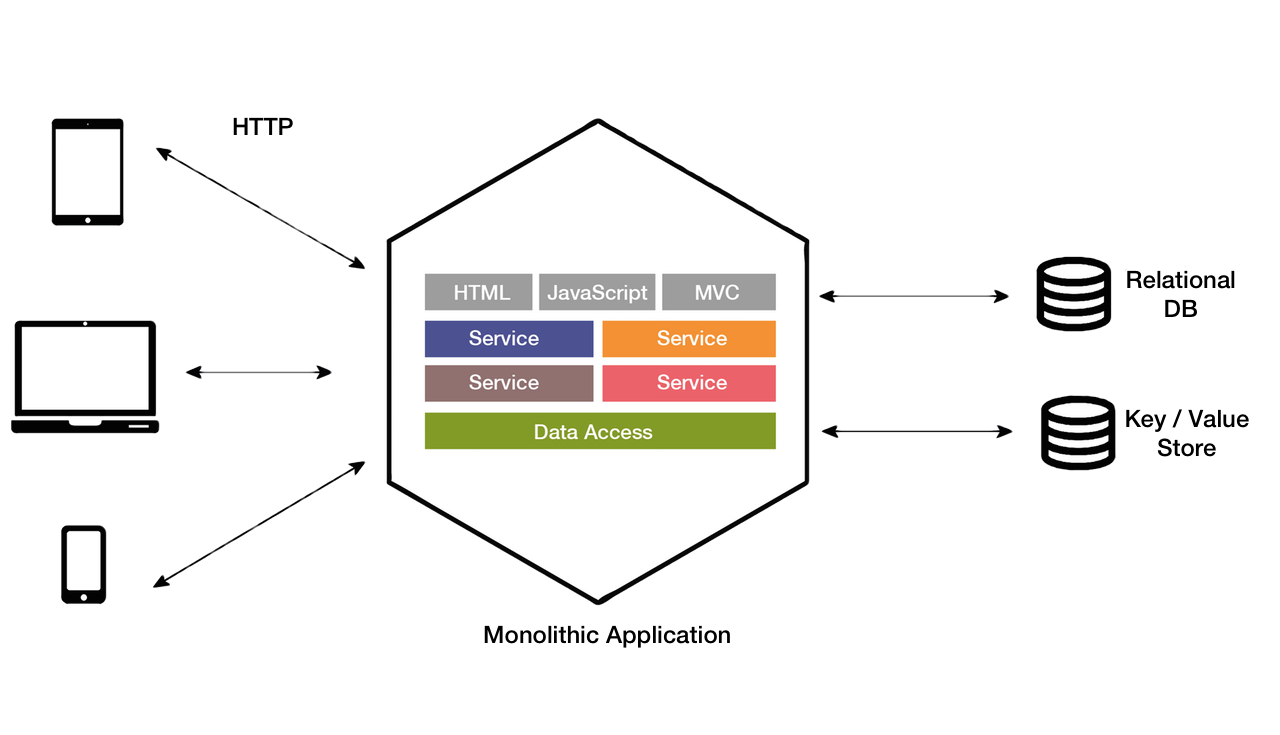
\includegraphics[scale=.2]{monolitFigure}
	\caption{Arhitectură Aplicație Monolit(imagine : http://bits.citrusbyte.com)}  
	\label{monolithicArhitecture}
  	\end{figure}
  	\section{Avantaje și dezavantaje}
  	\paragraph{}O aplicație monolit are mai multe avantaje in contextul unui business mic:
  	
  	\begin{itemize}
  	\item Faza de dezvoltare durează mai puțin timp, IDE-urile moderne reușind să genereze mult cod automat, ceea ce implică scădearea costurilor de producție.
  	\item Aplicația este usor de testat, automatizând procesul de testare a codului folosind o combinație de unit tests și integration test. 
  	\item Procesul de lansare în producție a unei aplicatii nu este complicat, deoarece este nevoie de rularea unei singure aplicații per server.
  	\end{itemize}
  	\paragraph{}Pe de altă parte, in momentul în care aplicația va creste ca și volum al codului, un număr mai mare de programatori vor trebui implicați în procesul de dezvoltare al aplicației, acest lucru nu este un lucru rău, doar ca aceștia vor intampina anumite impedimente:
  	\begin{itemize}
  	\item Cuplajul dintre componentele aplicației creste, iar acest fapt va îngreuna procesul de dezvoltare a unor noi functionalități, acest lucru va afecta timpul si costul necesar dezvoltării noii funcționalități.  
	\item Alegerea tehnologiilor folosite pentru dezvoltarea aplicației este permanentă.
	\item Integrarea/Intrarea unui programator in proiect va fi mai dificilă. Volumul aplicației fiind mare, va fi necesar un timp mai mare pentru înțelegerea tuturor funcționalităților si a decizilor luate pe proiect in trecut.
  	\end{itemize}
  	\paragraph{}Acestea sunt doar câteva dintre avantajele si dezavantajele unei aplicații monolit, dar sunt suficiente incât putem sublinia o idee generală. Aplicațiile bazate pe o arhitectura monolit sunt mai ușor de implementat în primă fază cu un cost mai redus, dar în momentul în care aplicația ajunge la un nivel mai avansat, este nevoie de o reconstruire parțiala sau totală a aplicației sau cel puțin este nevoie de o refactorizare care sa diminueze dezavantajele create de stilul arhitectural folosit. Majoritatea aplicațiilor încep ca și aplicații tip monolit, iar mai târziu se pot transaforma in aplicații cu arhitecturi bazate pe microservicii de exemplu.(\cite{thones2015microservices})
  \chapter{Arhitectura bazată pe servicii}
  	\section{Fundamentele arhitecturii bazate pe servicii}
  	\section{Sabloane de proiectare pentru arhitecturi bazate pe servicii}
  
\chapter{Sabloane de proiectare bazate pe microservicii}
	\section{Sabloane de implementare a microservicilor}
		\subsection{Agregator}
		\subsection{API Gateway}
	\section{Sabloane arhitecturale de proiectare}
		\subsection{Service bus}
		\subsection{Procesare asincrona}
		\subsection{Agregarea proceselor}
		\subsection{Alte Sabloane}
\chapter{Studiu de Caz}
	\section{Introducere}
	\paragraph{}Netflix este o companie care a început prin a vinde sau închiria filme pe DVD-uri. Ulterior furnizând acces online la filme si seriale. Netflix fiind un gigant in industria televiziunii online. Aplicația netflix este o aplicație la scară mondială, care în momentul in care firma a horărat schimbarea arhitecturii avea un trafic de 8 milioane de utilizatori, ajungând la finalul anul 2018 la 139 de milioane de utilizatori.	
	\paragraph{}Dupa cum am discutat până acum, o arhitectură bazată pe microservicii nu are chiar o definiție propriu zisă, dar dupa cum susține Martin Fowler, microserviciile sunt implementarea corectă a arhitecturii bazate pe servicii.
	\paragraph{}În acest capitol vom cuprinde trecerea de la o arhitectură monolit la o arhitectura bazată pe servicii, motivele pentru care s-a facut aceasta tranziție, pașii prin care s-a facut aceasta trecere, avantajele cât si dezavantajele acestei treceri, cât si despre rezultatul final.
	\section{Tranziția către microservicii (Netflix)}
	\paragraph{}În acest studiu de caz o să ne bazăm pe informațiile oferite de doua dintre personajele importante care au luat parte la tranziția catre microservicii:
	\begin{itemize}
	\item Ruslan Meshemberg
	\item Adrian Cockcroft	
	\item Josh Evans	
	\end{itemize}
	\subsection{Arhitectura aplicației de azi}
	\paragraph{}În următoarea diagrama, este reprezentată, arhitectura bazată pe microservicii a aplicației Netflix.
	\begin{figure}[h]
  	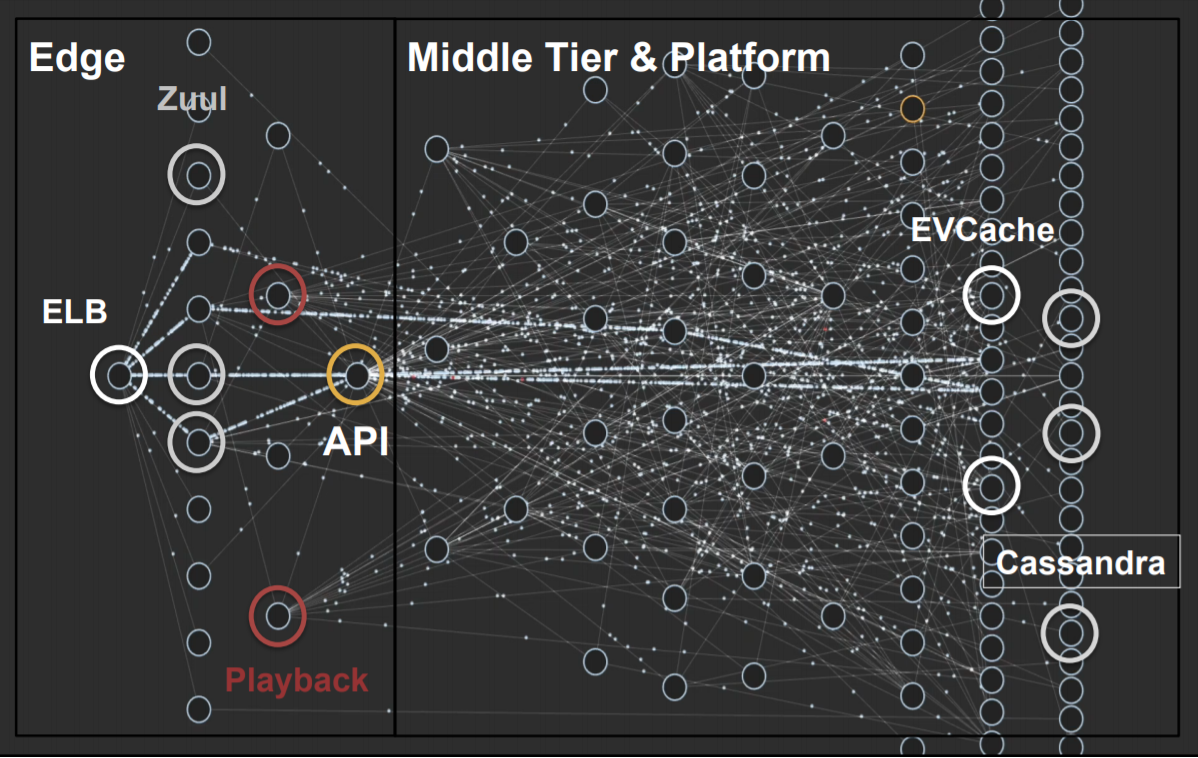
\includegraphics[scale=.651]{netflixarhitecuture}
	\caption{Arhitectura Aplicației Netflix()}  
  	\end{figure}
  	\paragraph{}Făcând o scurtă analiză asupra diagramei, putem să observam că prezentarea este una stratificată, nodul notat „ELB” rebrezintă un balansier de capacitate elastic (Elastic Load Balancer), care se o ocupă cu distrubuirea uniforma a cererilor catre microservicii. Stratul in care avem nodul notat „Zuul”, este un strat de tip proxy care ajută la oprirea atacurilor cibernetice. Iar zona dintre acest strat si „Middle Tier” este reprezentată de componente accesibile clientilor. În partea a 2-a a diagramei, este un strat destul de stratificat de microservicii care conțin mai multa logică si serversc componentelor din prima parte a diagramei. Ultimul strat, cel care contine si nodul notat cu „Cassandra” pe diagramă, reprezintă stratul de acces la bazele de date, datele fiind salvate separat in baza de date NoSQL. Iar intre ultimele 2 straturi   explicate, avem un strat care se ocupa de caching.
  	\paragraph{}O diagramă mai reprezentativă pentru arhitectura bazată pe microservicii a Netflix, care contine mai mult de 500 de microservicii este numita si diagrama de arhitectura „Death Star”(\ref{deathStarArhitecture}).
  	\paragraph{}Așadar, având în vedere scala la care știm deja ca funcționează aplicația Netflix, putem deja considera că arhitectura bazată pe microservicii isi servește bine scopul. În continuare vom discuta efectiv despre motivele, pașii, beneficiile și costurile acestei schimbari de arhitectură.
  	\begin{figure}[h]
  	\centering
  	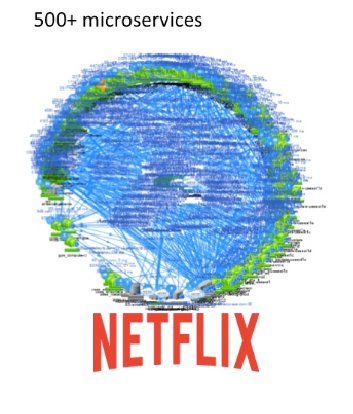
\includegraphics[scale=.8]{deathstararhitecture}
	\caption{Arhitectura Aplicației Netflix()}  
	\label{deathStarArhitecture}
  	\end{figure}
	\subsection{Motive}
	\paragraph{}Unul dintre primele motive care au înpins compania netflix isi mute aplicația catre cloud și odata cu asta, inceperea tranziției catre noua arhitectură, a fost o criza întampinata in 2008 când baza de date a fost coruptă, iar acest lucru a dus la intreruperea activitații timp de 3 zile. 
	\subsection{Avantaje și dezavantaje, costuri și sacrificii}
\chapter{Aplicație Practica}
	\section{Cerința}
	\section{Specificații}
	\section{Arhitectura aplicatiei}
	\section{Implementare}
	\section{Sablone bazate pe microservicii in practica}
\chapter{Concluzii}

\bibliographystyle{apacite}
\bibliography{referinte}

\begin{flushleft}
\textbf{Cockcroft, Adrian. 2015. \texttt{Talking microservices with the man who made Netflix’s cloud famous. [interviu cu] Derrick Harris. 2015.}}
\end{flushleft}

\begin{flushleft}
\textbf{
Cockroft, Adrian. 2014. \texttt{Migrating to Microservices by Adrian Cockroft. YouTube. [Interactiv] 2014. https://www.youtube.com/watch?v=1wiMLkXz26M.}}
\end{flushleft}

\begin{flushleft}
\textbf{
Erl, Thomas. 2009. \texttt{SOA Design Patterns. Crawfordville Indiana : Prentice Hall, 2009.}}
\end{flushleft}

\begin{flushleft}
\textbf{
Fowler, Martin. 2014. \texttt{Microservices, 2014,. MartinFowler.com. [Interactiv] 2014. https://martinfowler.com/articles/microservices.html.}}
\end{flushleft}

\begin{flushleft}
\textbf{
OASIS Foundation. 2006. \texttt{Reference Model for Service Oriented Architecture. [Interactiv] 2006. https://docs.oasis-open.org/soa-rm/v1.0/soa-rm.html.}}
\end{flushleft}



\end{document}
